\subsection{Error rate scaling}
\begin{figure}[t]
  \begin{subfigure}{.49\textwidth}
    \centering
    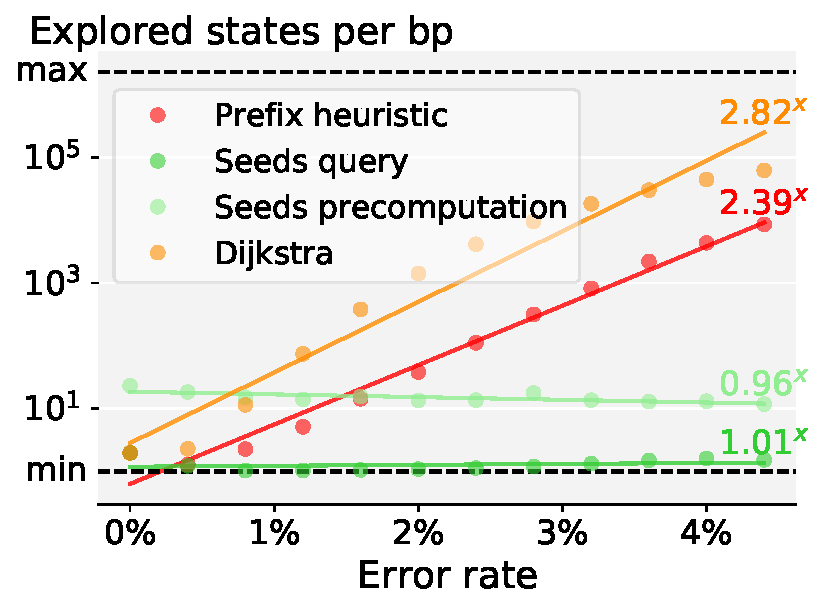
\includegraphics[width=\linewidth]{figures/prefix_vs_seeds_ecoli_250_errors_intervals_cmp_error_rate-explored_per_bp.pdf}
  \end{subfigure}%
  \begin{subfigure}{.45\textwidth}
    \centering
    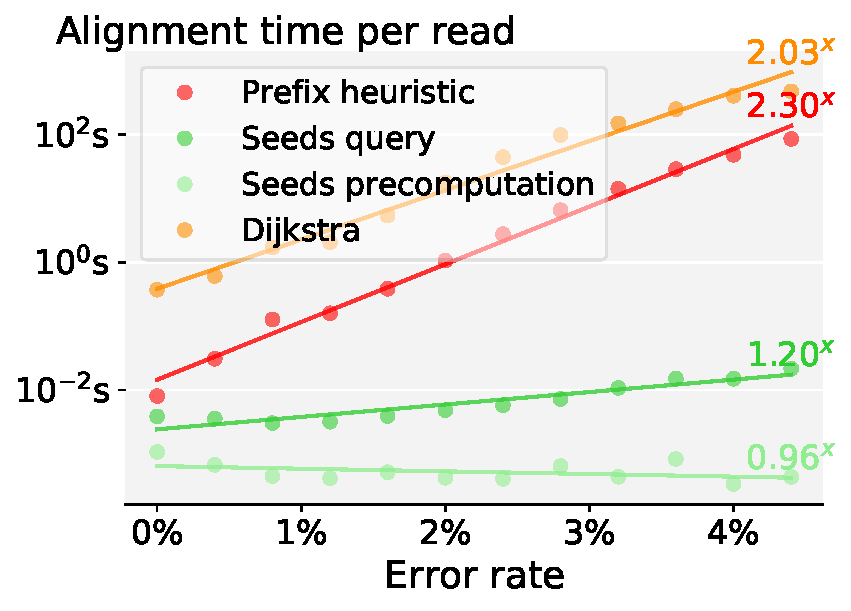
\includegraphics[width=\linewidth]{figures/prefix_vs_seeds_ecoli_250_errors_intervals_cmp_error_rate-t(map).pdf}
  \end{subfigure}~\hspace{1em} \caption{Average runtime and explored states
  comparison between \dijkstra, \prefixh and \seedh (precomputation and query)
  in respect to the error rate of Illumina 250bp reads on \textit{E.~coli}
  reference. The \seedh precomputation formally considers reference nodes which
  we refer to generalized states on the left plot. \todo{redo the experiment;
  make sure that one asymptotic fits the other data}}
  \label{SEEDfig:scaling_with_errorrate}
\end{figure}

Unlike the DP approaches which explore all states of the alignment graph, the \A
are sensitive to the alignment cost. In order to evaluate the scaling
characteristis of the \seedh, we compare the average alignment time of a read
dependent on its alignment cost. We simulated 400 PacBio CCS reads (with typical
read length between 200bp and 1000bp) using \randomreads.
\cref{SEEDfig:scaling_with_errorrate} compares \seedh and \prefixh on the Ecoli
genome. The \prefixh scales as $2.4^c$ whereas \seedh scales as $1.2^c$, where
$c$ is the alignment cost. Note that this is an exponential speed-up bringing
the base close to 1 which shows that the runtime is weakly dependent from the
alignment cost.
\todo{Comment that error rate scaling is limited for relatively low error rates.}
%$y = \lvert \{ \st{*}{x} \in \mli{Explored} \} \rvert$.

Linear best fit is according to SSD in the log space and with corresponding exponents.

\cref{SEEDfig:crumbs_by_errorrate} shows the average number of crumbs per read that
were added to the reference graph in relation to the error rate. The decrease in
the number of crumbs with read error rate is explained by the lower number of
seeds that match exactly in the graph.